%% This is file `elsarticle-template-5-harv.tex',
%%
%% Copyright 2009 Elsevier Ltd
%%
%% This file is part of the 'Elsarticle Bundle'.
%% ---------------------------------------------
%%
%% It may be distributed under the conditions of the LaTeX Project Public
%% License, either version 1.2 of this license or (at your option) any
%% later version.  The latest version of this license is in
%%    http://www.latex-project.org/lppl.txt
%% and version 1.2 or later is part of all distributions of LaTeX
%% version 1999/12/01 or later.
%%
%% The list of all files belonging to the 'Elsarticle Bundle' is
%% given in the file `manifest.txt'.
%%
%% Template article for Elsevier's document class `elsarticle'
%% with harvard style bibliographic references
%%
%% $Id: elsarticle-template-5-harv.tex 159 2009-10-08 06:08:33Z rishi $
%% $URL: http://lenova.river-valley.com/svn/elsbst/trunk/elsarticle-template-5-harv.tex $
%%
\documentclass[preprint,authoryear,12pt]{elsarticle}

%% Use the option review to obtain double line spacing
%% \documentclass[authoryear,preprint,review,12pt]{elsarticle}

%% Use the options 1p,twocolumn; 3p; 3p,twocolumn; 5p; or 5p,twocolumn
%% for a journal layout:
%%\documentclass[final,authoryear,1p,times]{elsarticle}
%%\documentclass[final,authoryear,1p,times,twocolumn]{elsarticle}
%%\documentclass[final,authoryear,3p,times]{elsarticle}
%%\documentclass[final,authoryear,3p,times,twocolumn]{elsarticle}
%%\documentclass[final,authoryear,5p,times]{elsarticle}
%%\documentclass[final,authoryear,5p,times, twocolumn, 12pt]{elsarticle}


%% if you use PostScript figures in your article
%% use the graphics package for simple commands
%% \usepackage{graphics}
%% or use the graphicx package for more complicated commands
\usepackage[demo]{graphicx}
\graphicspath{ {figura/} }
%% or use the epsfig package if you prefer to use the old commands
%%\usepackage{epsfig}

\usepackage[export]{adjustbox}
\usepackage{float}
\usepackage{dblfloatfix}
\usepackage{lipsum}
\usepackage{multicol}
\setlength{\columnsep}{1cm}
%%\setlength{\columnseprule}{1pt}
%%\usepackage{geometry}
%%\geometry{legalpaper, landscape, margin=2in}
\usepackage[a4paper, total={7in, 9in}]{geometry}


%% The amssymb package provides various useful mathematical symbols
\usepackage{amssymb}
%% The amsthm package provides extended theorem environments
%% \usepackage{amsthm}

%% The lineno packages adds line numbers. Start line numbering with
%% \begin{linenumbers}, end it with \end{linenumbers}. Or switch it on
%% for the whole article with \linenumbers after \end{frontmatter}.
%% \usepackage{lineno}

%% natbib.sty is loaded by default. However, natbib options can be
%% provided with \biboptions{...} command. Following options are
%% valid:

%%   round  -  round parentheses are used (default)
%%   square -  square brackets are used   [option]
%%   curly  -  curly braces are used      {option}
%%   angle  -  angle brackets are used    <option>
%%   semicolon  -  multiple citations separated by semi-colon (default)
%%   colon  - same as semicolon, an earlier confusion
%%   comma  -  separated by comma
%%   authoryear - selects author-year citations (default)
%%   numbers-  selects numerical citations
%%   super  -  numerical citations as superscripts
%%   sort   -  sorts multiple citations according to order in ref. list
%%   sort&compress   -  like sort, but also compresses numerical citations
%%   compress - compresses without sorting
%%   longnamesfirst  -  makes first citation full author list
%%
%% \biboptions{longnamesfirst,comma}

% \biboptions{}

%\journal{Nuclear Physics B}
\journal{Computers, Environment and Urban Systems}

\begin{document}

\begin{frontmatter}

%% Title, authors and addresses

%% use the tnoteref command within \title for footnotes;
%% use the tnotetext command for the associated footnote;
%% use the fnref command within \author or \address for footnotes;
%% use the fntext command for the associated footnote;
%% use the corref command within \author for corresponding author footnotes;
%% use the cortext command for the associated footnote;
%% use the ead command for the email address,
%% and the form \ead[url] for the home page:
%%
%% \title{Title\tnoteref{label1}}
%% \tnotetext[label1]{}
%% \author{Name\corref{cor1}\fnref{label2}}
%% \ead{email address}
%% \ead[url]{home page}
%% \fntext[label2]{}
%% \cortext[cor1]{}
%% \address{Address\fnref{label3}}
%% \fntext[label3]{}

%\title{}
\title{Proposta de Infraestrutura de Dados Espaciais para o Setor El\'etrico no Brasil\tnoteref{t1}}
\tnotetext[t1]{Artigo para Qualifica\c{c}\~ao de Mestrado no Programa de P\'os Gradua\c{c}\~ao em Geografia}
%% use optional labels to link authors explicitly to addresses:
%% \author[label1,label2]{<author name>}
%% \address[label1]{<address>}
%% \address[label2]{<address>}

%\author{}
\author{Candido, D. S.\corref{cor1}}
\ead{diogosantana@aneel.gov.br}
\ead[url]{sigel.aneel.gov.br}

\author{Carvalho Junior, O. A\corref{cor2}}
\ead{osmarjr@unb.br}

%\address{}
\address{Universidade de Bras\'{\i}lia, Instituto de Ci\^encias Humanas, Departamento de Geografia, Bras\'{\i}lia, DF - Brasil}


\cortext[cor1]{Aluno de Mestrado}
\cortext[cor2]{Professor Orientador}


\begin{abstract}
%% Text of abstract

\end{abstract}

\begin{keyword}
%% keywords here, in the form: keyword \sep keyword

%% MSC codes here, in the form: \MSC code \sep code
%% or \MSC[2008] code \sep code (2000 is the default)

\end{keyword}

\end{frontmatter}

% \linenumbers
%% main text
%\section{}
\section{Introdu\c{c}\~ao}
\label{sec1}
\begin{multicols}{2}
Com o advento e populariza\c{c}\~ao do Sistema de Infoma\c{c}\~ao Geogr\'afica (SIG) aliado com os avan\c{c}os decorrentes da evolu\c{c}\~ao da Tecnologia da Informa\c{c}\~ao e Comunicação (TIC) ocorrido nos \'ultimos anos, existe uma crescente demanda pela utiliza\c{c}\~ao das Informa\c{c}\~oes Geoespaciais (IG) abrangendo os mais diversos stakeholders em diferentes setores da sociedade \citep{Macharis2014AFlanders, Kounadi2016AdaptiveDatasets}.



Para a utilização das IG de forma eficiente e eficaz necessita-se que a organização desses específicos tipos de dados obedeça aos padrões e normas referentes a uma Infraestrutura de Dados Espaciais (IDE), que pode ser conceituada como um conjunto de políticas, padrões, tecnologia e acordos institucionais para o acesso, compartilhamento e organização das IG \citep{DAmore2012ICTManagement, Kobben2013TowardsInfrastructure, Stock2012ToInfrastructure}.
Quanto à classificação referente ao tipo de escala de implementação a IDE pode ser classificadas nos níveis: Global, Continental, Nacional, Regional, Local, Organizacional ou até mesmo Departamental, essa escolha vai depender basicamente do seu público alvo e do tipo de informação que a IDE vai organizar \citep{Bejar2012AnInfrastructures}, já quanto ao seu enfoque pode ser visto por dois pontos diferentes: O primeiro no nível mais Corporativo abrangendo os acordos institucionais, definição de políticas, normas e regulamentação para a sua implementação nas instituições, ocupando um nível de análise mais estratégico e o segundo pode ser analisado num nível mais Técnico abrangendo definição e especificação dos serviços de mapas e protocolos web, modelagem de dados e catálogos de metadados, ocupando um nível mais Operacional \citep{Cooper2013AViewpoint}. 
Em regra, uma IDE está sob controle de uma entidade governamental que pode ser a entidade responsável pela produção, aquisição, manutenção, gerenciamento e compartilhamento deste específico tipo de IG, ou mesmo a entidade que atue apenas no campo político e administrativo \citep{Grus2011AnGoals}, essa heterogeneidade na administração e produção dos dados prejudica a interoperabilidade, limitando a utilização desses dados pelas diferentes corporações. Nos últimos anos, o conceito de governança através de práticas relacionadas à boa gestão dos recursos tem sido evidenciado pelas principais entidades, não muito diferente o Setor Público necessitou também de evoluir para melhorar a prestação de serviços públicos para a sociedade, neste cenário com o avanço da TIC e sob o conceito de e-Government que pode ser definido como as iniciativas do Governo Eletrônico para facilitar o acesso à informação para a sociedade, ampliando as discussões sobre a prestação dos serviços públicos com enfoque na sua eficácia e efetividade \citep{Borzacchiello2013EstimatingE-Cadastres}, as IDEs apresentam-se como importante ferramenta para realizar o aumento da eficácia e efetividade na utilização de recursos públicos.
Este artigo está organizado da seguinte maneira: Na seção 1, realiza um apontamento para a importância de uma IDE apresentando seus principais conceitos e definições já na seção 2 apresentam as definições e conceitos da Infraestrutura Nacional de Dados Espaciais (INDE) existente no Brasil e destacando seus componentes. Na seção 3, ocorre o detalhamento do componente de Energia da INDE e na seção 4 apresenta uma proposta de implementação de uma IDE na componente de Energia, seguindo da sua Discussão e Conclusão.
\end{multicols}

\section{Infraestrutura Nacional de Dados Espaciais no Brasil}
\label{sec2}
Texto

\section{Infraestrutura de Dados Espaciais no Setor El\'etrico}
\label{sec3}
Texto

\section{Metodologia para implantar uma Infraestrutura de Dados Espaciais}
\label{sec4}

\begin{figure}[H]
    \centering
    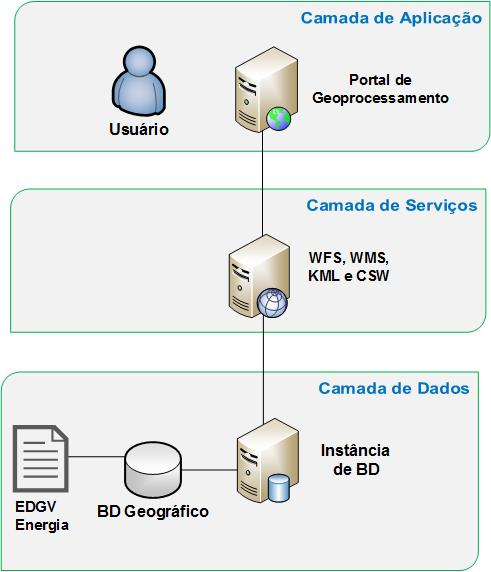
\includegraphics[scale=0.7]{fig3}
    \caption{Arquitetura IDE Energia}
    \label{fig:my_label}
\end{figure}

\section{Resultados}
\label{sec5}


Texto



\begin{figure}[H]
\centering
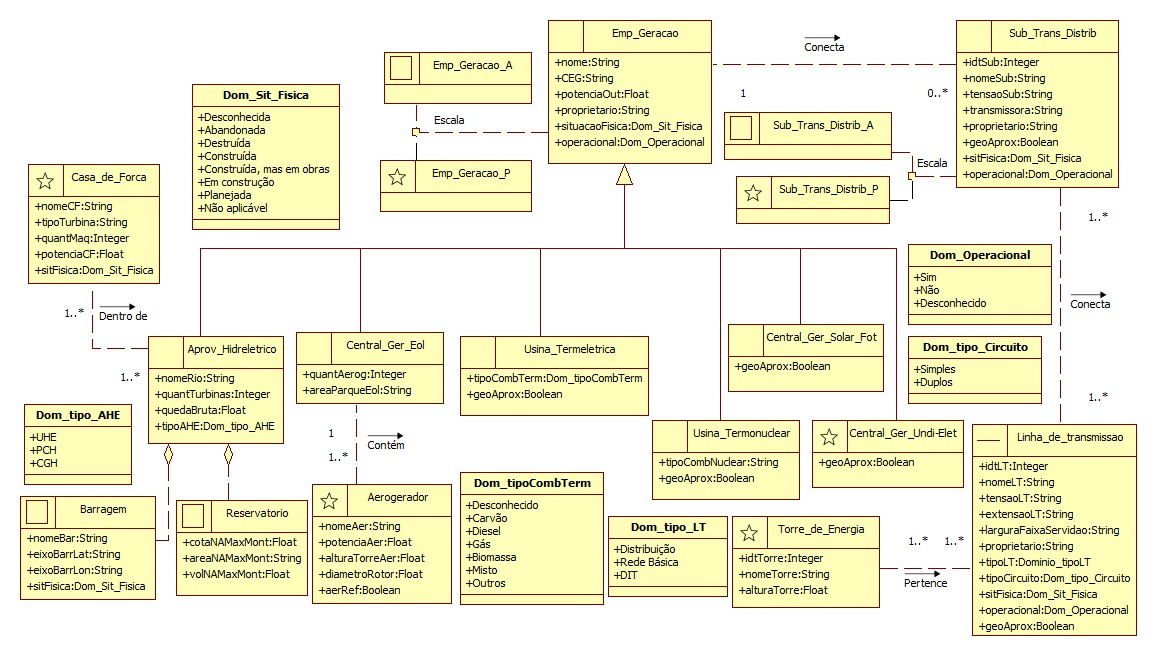
\includegraphics[width=\textwidth]{fig} 
\caption{Modelagem Conceitual do Tema Energia}
\label{fig:subim1}
\end{figure}

\section{Discuss\~ao}
\label{sec6}
Texto

\section{Conclus\~ao}
\label{sec7}
Texto

\appendix
\section{Descri\c{c}\~ao dos atributos}
\label{appendix}

%% The Appendices part is started with the command \appendix;
%% appendix sections are then done as normal sections
%% \appendix

%% \section{}
%% \label{}

%% References
%%
%% Following citation commands can be used in the body text:
%%
%%  \citet{key}  ==>>  Jones et al. (1990)
%%  \citep{key}  ==>>  (Jones et al., 1990)
%%
%% Multiple citations as normal:
%% \citep{key1,key2}         ==>> (Jones et al., 1990; Smith, 1989)
%%                            or  (Jones et al., 1990, 1991)
%%                            or  (Jones et al., 1990a,b)
%% \cite{key} is the equivalent of \citet{key} in author-year mode
%%
%% Full author lists may be forced with \citet* or \citep*, e.g.
%%   \citep*{key}            ==>> (Jones, Baker, and Williams, 1990)
%%
%% Optional notes as:
%%   \citep[chap. 2]{key}    ==>> (Jones et al., 1990, chap. 2)
%%   \citep[e.g.,][]{key}    ==>> (e.g., Jones et al., 1990)
%%   \citep[see][pg. 34]{key}==>> (see Jones et al., 1990, pg. 34)
%%  (Note: in standard LaTeX, only one note is allowed, after the ref.
%%   Here, one note is like the standard, two make pre- and post-notes.)
%%
%%   \citealt{key}          ==>> Jones et al. 1990
%%   \citealt*{key}         ==>> Jones, Baker, and Williams 1990
%%   \citealp{key}          ==>> Jones et al., 1990
%%   \citealp*{key}         ==>> Jones, Baker, and Williams, 1990
%%
%% Additional citation possibilities
%%   \citeauthor{key}       ==>> Jones et al.
%%   \citeauthor*{key}      ==>> Jones, Baker, and Williams
%%   \citeyear{key}         ==>> 1990
%%   \citeyearpar{key}      ==>> (1990)
%%   \citetext{priv. comm.} ==>> (priv. comm.)
%%   \citenum{key}          ==>> 11 [non-superscripted]
%% Note: full author lists depends on whether the bib style supports them;
%%       if not, the abbreviated list is printed even when full requested.
%%
%% For names like della Robbia at the start of a sentence, use
%%   \Citet{dRob98}         ==>> Della Robbia (1998)
%%   \Citep{dRob98}         ==>> (Della Robbia, 1998)
%%   \Citeauthor{dRob98}    ==>> Della Robbia

\begin{multicols}{2}
%% References with bibTeX database:
\bibliographystyle{model5-names}
\bibliography{mendeley}

%% Authors are advised to submit their bibtex database files. They are
%% requested to list a bibtex style file in the manuscript if they do
%% not want to use model5-names.bst.

%% References without bibTeX database:

% \begin{thebibliography}{00}

%% \bibitem must have one of the following forms:
%%   \bibitem[Jones et al.(1990)]{key}...
%%   \bibitem[Jones et al.(1990)Jones, Baker, and Williams]{key}...
%%   \bibitem[Jones et al., 1990]{key}...
%%   \bibitem[\protect\citeauthoryear{Jones, Baker, and Williams}{Jones
%%       et al.}{1990}]{key}...
%%   \bibitem[\protect\citeauthoryear{Jones et al.}{1990}]{key}...
%%   \bibitem[\protect\astroncite{Jones et al.}{1990}]{key}...
%%   \bibitem[\protect\citename{Jones et al., }1990]{key}...
%%   \harvarditem[Jones et al.]{Jones, Baker, and Williams}{1990}{key}...
%%

% \bibitem[ ()]{}

% \end{thebibliography}
\end{multicols}
\end{document}

%%
%% End of file `elsarticle-template-5-harv.tex'.
